\chapter{Introduction to the CoreASIM Language, Interpreter, and ICEF}
\label{ch:CoreAsimIntro}

\vspace{-1cm}
\begin{center}
Eduard Hirsch
\end{center}

This chapter provides an overview of the technologies used for running the INTERLACE Specification. At the beginning a quick-start description is provided in order make it easier to jump right into the execution of the model. Additional details about how the executable models of Abstract State Interaction Machine (ASIM) specifications function in the environment are discussed, along with how this can happen in a simple and stable manner.

There are two base environments available -- one based on Docker (henceforth `docker') and one based on Vagrant (henceforth `vagrant'). During project execution, the focus shifted from the vagrant environment, which can be downloaded from GitHub,\footnote{\url{https://github.com/InterlaceProject/ASIMVagrantEnvironment}} to a docker-based version which is explained in Section \ref{sec:quick-start-docker} and is also available on GitHub.\footnote{\url{https://github.com/InterlaceProject/ASIMDockerEnvironment}} Nevertheless, the vagrant setup is still explained for those developers who prefer it.

\section{Quick-Start Vagrant}
\label{sec:quick-start-vagrant}

The vagrant definition provides a running environment for executing the INTERLACE ASIM definitions. During the provisioning process an Ubuntu vagrant box is set up. All the necessary components are installed in that box, which clones and builds the ICEF framework\footnote{\url{https://github.com/biomics/icef}} as well as the ASIM Specification\footnote{\url{https://github.com/InterlaceProject/ASIMSpec}} into the data directory where it is finally ready for use.

\subsection{Prerequisites}

Download and install the following software products:
\begin{itemize}
	\item Virtual Box: \url{https://www.virtualbox.org/}
	\item git: \url{https://git-scm.com/downloads}
	\item Vagrant: \url{https://www.vagrantup.com/}
\end{itemize}

\subsection{Clone Environment}

To clone the ASIM vagrant environment from github into a directory git can be utilized:
\begin{lstlisting}
	git clone https://github.com/InterlaceProject/ASIMVagrantEnvironment.git
\end{lstlisting}

\subsection{Execution}

Once all software components are installed and the vagrant definitions are cloned it is possible to call

\begin{lstlisting}
	execute.sh
\end{lstlisting}

from the main directory in order to run the INTERLACE specifications. Note: when using Windows it is necessary to start that command within git-bash which needs to run in elevated admin mode (right click $\rightarrow$ start as administrator). That is necessary to handle symbolic links in git-bash.

On the very first execution the script is provisioning a virtual machine based on Ubuntu by calling \textit{vagrant up}, which may take some time. Subsequent calls will be much faster. A detailed description explaining the precise process is covered in Section \ref{sec:exec-env-model-details}.

Once the execution is started it will run until it is stopped by pressing \textbf{ctrl + c} or by calling
\begin{lstlisting}
	stop.sh
\end{lstlisting}
from any other console window.

\section{Quick-Start Docker}
\label{sec:quick-start-docker}

The docker project on GitHub\footnote{\url{https://github.com/InterlaceProject/ASIMDockerEnvironment}} is also based on virtualization like the vagrant environment, but emphasizes \textit{Operating System virtualization} instead of \textit{Hardware virtualization} \cite{VirtualMachines2005}.

\subsection{Prerequisites}

\begin{itemize}
	\item install docker
	\item install git (including git bash for windows)
\end{itemize}
On Linux machines it is important to add the current user to the docker group in order to manage docker container and images. Otherwise all further explained commands need to be executed as root or with sudo.

For Windows machines use \textit{git-bash} to execute the commands described in the following sections.

\subsection{Before First Execution}

In order to configure the environment it is necessary to call the following script:
\begin{lstlisting}
	./configure
\end{lstlisting}
This will generate a docker container image called \textit{asim} where all the necessary frameworks are built and prepared for execution of the specifications. The ICEF framework as well as the ASIM model specifications are cloned outside of the container to simplify development.

\subsection{Execute Specification}
The container image \textit{asim} created during the configuring step can be started by calling
\begin{lstlisting}
	./execute
\end{lstlisting}
A container started in this way is called \textit{active\_asim} and runs all the necessary steps, like starting an ICEF manager as well an ICEF brapper to run the ASIM specifications.

Like the vagrant environment, a running execution may be stopped by pressing \textbf{ctrl + c}.

\section{Execution Environment Stack}
\label{sec:exec-env-stack}
Regardless of the virtualization techniques used, a consistent base system is used. Therefore, both docker and vagrant are provisioning a Linux-based operating system. In this case the Ubuntu 16.04 LTS (Long Term Support) distribution is facilitated. That consistent, stable and reliable structure will be important later when considerations about provability as well as testability become relevant; namely, that design always provides the same preconditions and anybody executing or testing against the specification will obtain the same results.

\subsection{Software Stack}
\label{sec:env-exec-stack-software-stack}

The Ubuntu 16.04 LTS distribution is enhanced and updated according to the needs of an ASIM executing machine as well as to the needs of developers working with that virtual system. To be more specific the following components are installed during the provisioning process:

\begin{itemize}
	\item \textbf{curl} $\rightarrow$ Is a tool for querying REST resources and used for downloading packages from various online repositories.
	\item \textbf{nodejs} $\rightarrow$ Is a JavaScript runtime environment built on Chrome's V8 engine and includes the package manager npm. This bundle is necessary for installing and running the Manager component of ICEF.
	\item \textbf{build-essential} $\rightarrow$ These packages are needed to compile a debian-based package and provide help for building \textcolor{red}{(compiling, etc)} the project sources.
	\item \textbf{maven} $\rightarrow$ Is a well-known Java build and packaging tool and used for building the ICEF framework as well as the coreASIM Eclipse plugin.
	\item \textbf{vim} $\rightarrow$ Well-known U/Linux editor which acts as helper for quick development or configuration issues inside the environment.
	\item \textbf{git} $\rightarrow$ Distributed Version-Control System which helps downloade source repositories from GitHub.
	\item \textbf{Java 8} $\rightarrow$ Programming Language used for coreASIM's base system implementation; thus, also for running ASIM instances.
\end{itemize}

\subsection{Provisioning Process}

The provisioning process can be separated into 3 steps which are executed when \textit{.\/configure} for docker or \textit{vagrant up} for vagrant is called from the command line:

\begin{enumerate}
	\item Download ASIMSpec and ICEF from GitHub
	\item Install of software packages mentioned in Section \ref{sec:env-exec-stack-software-stack}
	\item Build the ICEF framework and prepare a virtual machine for execution
\end{enumerate}

For development purposes the ASIMSpec and the ICEF frameworks are cloned into directories which are available from the host machine and the virtual guest machine. This is necessary because then it is possible to directly edit the source or debug from outside and execute the code from within the container. Consequently it is not necessary to copy the code into the container when changes are carried out.

For \textbf{vagrant}, a shared folder is configured over the vagrant file shown here:
\begin{lstlisting}
	...
	config.vm.synced_folder "./data", "/vagrant-data"
	...
\end{lstlisting}
\textcolor{red}{This command} refers to the fact that the folder \textit{data} is used on the host system and a folder \textit{vagrant-data} is mounted on the guest system. These folders are shared and thus contain the same content. Additionally, during provisioning a symbolic link in the home directory is created called project (\textit{/home/ubuntu/project}), which links the mounted root folder /vagrant-data.

When the virtual machine is stopped the data directory on the host is kept and can be still manipulated or executed (of course only if the framework dependencies are installed on the host as well).

For \textbf{docker}, first all GitHub sources need to be cloned to the host machine, and only then can files be shared into the guest container by using the command line option "-v"
\begin{lstlisting}[language=bash]
	docker run -v "$1/ASIMSpec:/home/ASIMSpec" \
	           -v "$1/icef:/home/icef" \
	           --name active_asim -it asim /$2
\end{lstlisting}

This line is part of the script \textit{scripts/runDocker.sh}. \$1 here stands for the local directory of the environment and \$2 is normally defaulted to the main execution script started inside the docker container. It is important to note that the \textit{ASIMSpec} folder of the host machine is shared into \textit{/home/ASIMSpec} of the docker container and the \textit{icef} directory is shared into \textit{/home/icef}.

\textcolor{red}{In the above paragraph you use `shared into' three times. I am not sure what you mean exactly. Normally something is shared \emph{with} something or someone, not \emph{into}. However, you might mean something more complicated, like a two-step process: for example, something is moved into a folder, and then it is also made shareable. Even in such a case, however, saying \emph{who} or \emph{what} the object is shareable with would help.}

\subsection{Execution}
\label{sec:env-exec-stack-exe}

The execution stack in Figure \ref{fig:icef-intro-asim} shows where a ICEF specification is transmitted for it to be executed. The details will be covered in Section \ref{sec:icef-intro}. In this part of the document we take a look at which services are started and how.

Due to limitations of the ICEF framework it is currently not possible to cleanly shut down a running ICEF simulation with several running ASIM instances. Therefore both environments have to start and stop all services for every execution in order to guarantee a correct execution set-up.

\subsubsection{Start Services Processes}.  Both environments offer a script that needs to be called from the host system (\textit{execute(.sh)}) and one that needs to be called from within the virtualized machine (\textit{executeASIMSpec.sh/executeOnGuest.sh}). Whereas the script on the virtualized system only differs in directory references the outside scripts have to handle different things as one script deals with docker and the other with vagrant.

In detail, docker can start the servers immediately and run the script inside the container, whereas vagrant needs to add an additional step if the virtual machine is not up and running yet. Thus, vagrant
\begin{enumerate}
\vspace{-0.5cm}
	\item tries to start the server processes and submit the specifications;
	\item if the first step fails, the script checks if the virtual machine is running. If it isn't, the script tries to (re-)start it;
	\item when the restart is successful the first step is retried.
\end{enumerate}

If we focus on the first step, which is basically the same in both environments, we can discuss in detail how the process continues. Thus, on the guest system we are first running a so-called \textit{CASIMA}, which is short for coreASIM-Manager \ref{sec:icef-intro}. This manager takes care of ASIM states, scheduling, and also acts as messaging backbone.

Next, a second service process is started. The service is a wrapper for the coreASIM implementation and its name is Brapper (BIOMICS wrapper). This Brapper service executes enhanced ASIM code named BSL that offers additional language primitives specifically designed during the BIOMICS project. Those features mainly include interaction features used to model biochemical systems. Nevertheless, and actually because of that, they are also suitable for decentralized and distributed computational systems.

\textcolor{red}{When a Brapper starts, it needs to register with a manager instance.}
\st{When a Brapper is going to be started it needs to be register at a manager instance.}
As described in Section \ref{sec:icef-intro}, it is possible to start multiple Brappers. Once a simulation is submitted to the manager, the manager distributes the different simulations, including their ASIMs, to different Brapper services to execute them there, while trying to spread the load equally.

For the sake of simplicity the environment starts only one Brapper by default. In the final implementation it will be possible to specify the number of Brappers to be used for execution.

\subsubsection{Submit ICEF definition file}. Finally, after the service processes are running it is possible to submit a specification file to the manager. This is done by executing a bash script which calls a  nodejs client:

\begin{lstlisting}
	...
	node loadICEF.js $project/ASIMSpec/run.icef localhost 9090
	...
\end{lstlisting}

The above listing uses a \textit{\$project} variable containing the path of ASIMSpec to find the ICEF specification. By convention the ICEF definition file of the ASIM Specification is called \textit{run.icef} to clearly identify the entry point for the environment. The last two parameters for the script are the host and the port where the manager service is running and waiting for requests, respectively.

\subsection{Development}
\label{sec:development}
For developing new simulations it is important to have a proper development environment. There exist many different IDE/Tool/Debuggers choices for Java and JavaScript which may be used for the Brapper, Manager or coreAS(I)M plugin development. However, there are only limited IDE choices for implementing AS(I)Ms.

For the well-known Integrated Development Environment Eclipse, developers of the ICEF framework have adopted the coreASM plugin for supporting the additional language primitives. Thus for working with ASIM implementations of INTERLACE you ideally DO NOT download the coreASM plugin package which is available at the marketplace of Eclipse. \textcolor{red}{In the previous sentence you say that we do not use the coreASM plugin. In the sentence before that you say that we do. I am confused :) .} The adopted plugin working with the new language elements is provided by the ICEF framework directly but it needs to be built and imported manually into Eclipse.

\textbf{Import/Install of the IDE Eclipse plugin for coreASIM}
\begin{quote}
\small
\begin{description}
	\item[Build Framework.] To add the ASIM plugin to Eclipse the coreASIM plugin needs to be built and installed  manually first because it is not downloadable from the Eclipse marketplace and is only available as a source version delivered with the ICEF framework and as part of the coreASIM engine. Building and installing can be done by calling
	\begin{lstlisting}[language=bash]
		cd icef/coreASIM/org.coreasim.parent && mvn package install
		cd icef/coreASIM/org.coreasim.eclipse && mvn package install\end{lstlisting}
	Note that the ICEF directory is placed in different folders in the two environments!
	
	\item[Install Plugin Development Environment in Eclipse.] To install the ASIM plugin it is necessary to first add another plugin called Eclipse PDE (Plugin Development Environment) from the marketplace for the current Eclipse installation or get a distribution which already contains that plugin.
	
	\item[Import Plugin as Project.] Next, the plugin needs to be imported to the workspace, which can be done in Eclipse using the import wizard. To reach the wizard go to "File" $\rightarrow$ "Import...", search for "Existing Projects into Workspace" and click to get to "Import Project" Window. Then click "Finish" to import the project.
	
	\item[Dry-Run Eclipse with coreASIM Plugin.] This optional step can be done to check if the plugin is working correctly. For that it is possible to right-click the imported Eclipse project and go to ``Run As'' $\rightarrow$ "Eclipse Application". Then a second Eclipse instance is started but this time a new tab should appear named ``coreASIM''. In addition, when opening a file with extension \textit{casim} the ASIM definition should be syntax-highlighted.

	\item[Enable the Plugin.] If the (optional) dry-run has been successful the export wizard will export the plugin into the running Eclipse installation by opening "File" $\rightarrow$  "Export" then choosing "Deployable plugins and fragments" in the new Dialogue. The window which is opened next will offer to export fragment  \textit{org.coreasim.eclipse} by selecting the checkbox next to it. Before clicking "Finish", the combo box "Install into host" has to be chosen.
\end{description}
\end{quote}

Once these steps have been completed Eclipse will offer a new tab in the top menu bar called "CoreASIM" on restart.

\textbf{Note on the installation}: When using the \textit{docker}-Environment you could skip the first step \textbf{Build Framework}, because all the necessary build steps are covered by the initial configuration script. Also a separate installation of the Eclipse plugin Development Environment (PDE) might omitted because it usually comes in a bundle with most standard J2EE installations of Eclipse.

\textbf{Notes on the Docker Environment}
\label{sec_inner:note-docker}

Normally the ASIM Specifications are started by calling \textit{execute} from the main directory. This starts a script which will run the required services and then send the ICEF definition. When stopping the container it instantly goes back to its original state before execution. Only the shared directories ASIMSpec and ICEF will retain the changes.

If it is necessary or convenient, for example if the host is missing development packages (e.g.\ maven, nodejs, ... ) which are available inside the container, it is possible to work from within the container by calling
\begin{lstlisting}
	./execute /bin/bash
\end{lstlisting}
which starts the docker container, runs a bash shell instead of the starting script, keeps the STDIN open, and connects a pseudo TTY. In this way it is possible to work with the container's bash shell, which can be seen as analogous tos connecting to a remote shell over SSH.

\section{ICEF - The Interaction Computing Execution Framework}
\label{sec:icef-intro}

The interaction framework wraps the original coreASM framework in order to extend it and give it the capabilities to support concurrent and distributed computation. It was developed in a project called BIOMICS and financed by the European Commission.\footnote{\url{http://biomicsproject.eu/}}

\textbf{This wrapping took place on three levels:}
\begin{quote}
\vspace{-1.5cm}
\small
\textbf{First}, the interpreter coreASM had to be extended supporting additional language primitives as well as communications features. Here BSL replaces ASM as a new language having a new interpreter coreASIM.

\textbf{Second}, a space was created where the now so-called Abstract State Interaction Machines (ASIMs) take over and are able to execute in parallel. This environment is called Brapper (short for BIOMICS Wrapper).

\textbf{Third}, a central server called manager takes care of handling distributed Brapper instances, dealing with message and scheduling issues.
\vspace{-1cm}
\end{quote}

In terms of technology, the development of coreASIM involved making changes to the Java coreASM implementation. Brappers are written in Java as well but the managers coordinate the Brappers using nodejs and are therefore written in JavaScript.

\subsection{Framework Stack}

We now describe in more detail the aspects of the ICEF framework stack that concern the INTERLACE implementation. Figure \ref{fig:icef-intro-asim} shows the stack at different levels of granularity.

As a stable base for the INTERLACE execution environment stack we chose a Linux-based system, Ubuntu 16.04 LTS. A LTS (Long-Term Support) version is important to ensure thta we have a reliable platform that is maintained by the distributor for a long time. Ubuntu publishes LTS versions every two years and promises a maintenance duration of five years.\footnote{\url{https://www.ubuntu.com/info/release-end-of-life}}

After installation of the software described in Section \ref{sec:env-exec-stack-software-stack} and after building the ICEF components, the framework is ready. When the components are started it is possible to transmit a running definition, called ICEF JSON file.

Listing \ref{lst:icef-json-spec} shows what the specification for the simulation looks like. An \textit{id} for the simulation is given, along with one scheduler and one ASIM. The \textit{schedulers} section normally only hosts one scheduler which takes care of other active or suspended ASIM agents. The \textit{asims} attribute in the JSON file defines the actual ASIM instances running the simulation.

Side note: A definition for the client here is not given because the client which is sending credit, debit or other requests is spawned and destroyed on demand by the Scheduler ASIM defined in \textit{casim/scheduler.casim}.

Detailed descriptions of parameters and options of the JSON ICEF specifications can be found in Deliverable D5.2 \cite{BIOMICSD52} of the BIOMICS project.

\begin{minipage}{1.0\textwidth}
\begin{lstlisting}[language=json,firstnumber=1,caption={ICEF JSON Specification for INTERLACE},captionpos=b,label=lst:icef-json-spec]
{
   "id": "interlace", 
   "schedulers": [
       {
	   "file": "casim/scheduler.casim",
	   "start": true
       }
   ], 
   "asims": [       
       {
           "file": "casim/server.casim",
           "start": true
       }
   ]
}
\end{lstlisting}
\end{minipage}

The implementation idea here is to have a central server which takes over the various requests from the clients. A scheduler will take care of what exactly is running, and when. As a second task the scheduler will, as mentioned before, also spawn new clients which send or receive information/requests to other components, but mainly to the server.

\textbf{The Submission Process} of the \textit{run.icef} works as follows:

\begin{quote}
\small
\begin{description}
	\item [Loading and parsing of the ICEF-File] initializes the process. Using that specification file a node.js component transmits the structure to the manager server process which acts as the central managing and communication node.
	\item [Starting Simulation] on the manger service process. During that process the service registers a new simulation and all components necessary for managing the different resources like messaging.
	\item [Distribute ASIMs.] When simulations are initialized requests are sent to one or more Brappers in order to start up the actual running instances of the ASIM agent.
	\item [Run.] Finally, when all ASIM instances are running the simulation is successfully executing till stopped from the outside or by a problem during execution.
\end{description}
\end{quote}

\begin{figure}[htbp]
  \centering
  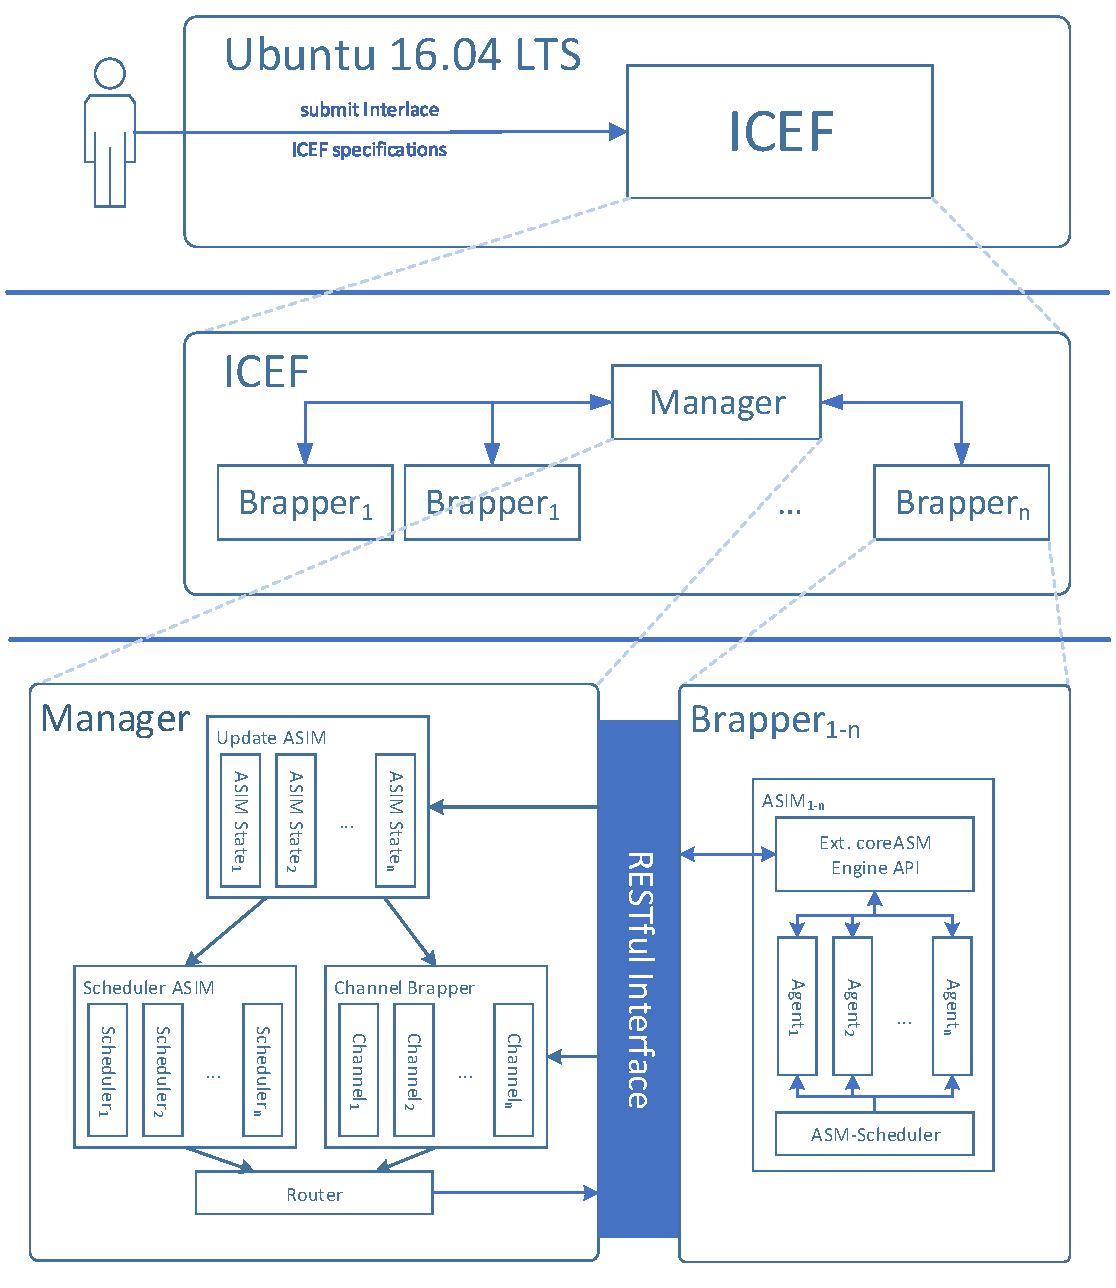
\includegraphics[width=1.0\textwidth, clip, trim=1mm 1mm 1mm 1mm]{Figures/environment_asim}
  \caption{\bf\small ASIM Execution Environment Overview}
  \label{fig:icef-intro-asim}
\end{figure}

Figure \ref{fig:icef-intro-asim} illustrates on different levels of detail which components and services are active and necessary to get the processes described above to run an ASIM simulation and, in the case of INTERLACE, the model specification.

\subsection{coreASIM}
\label{sec:coreasim-details}

The very core of the Interaction Computing Execution Framework (ICEF) is an engine which was developed by different people at different universities\footnote{\url{https://github.com/CoreASM/coreasm.core/wiki/About\-CoreASM}} and implements a language called ASM. This language is based on Abstract State Machines \cite{BoergerStaerk2003}, which is used as a methodology for high-level system engineering, design, and analysis. This engine, called coreASM, was enhanced by the BIOMICS project in order to simulate computer interactions on a logic-based programming language.

The resulting engine is called coreASIM and includes the interaction features that were missing in coreASM \cite{BIOMICSD42}\cite{BIOMICSD52}. CoreASIM replaces the ASM language with the BIOMICS Specification Language (BSL). The changes from the original framework also comprise of:

\begin{itemize}
	\item interaction possibilities
	\item abstract shared storage
	\item mailing system
	\item full scheduler
	\item interpreter enhancements
\end{itemize}

As this document provides an overview only on the coreASIM features, just the most important implementations are described here; namely, the mailbox and the scheduling system.

\textbf{The mailing system} is easy to use and can be described as follows:
\begin{quote}
\small
%\begin{minipage}{1.0\textwidth}
An ASIM $asim_1$ can send a message to another ASIM $asim_2$ by using the Send Message rule.\nopagebreak
\begin{lstlisting}[language=bsl]
	send Element to "asim_2" with subject "a subject"
\end{lstlisting}
Where the \textit{Element} can be any of the element locations used in the ASIM language space -- even, for example, \textit{program(self)}.
%\end{minipage}
\end{quote}

\textbf{The scheduler} has the ability to coordinate different local agents to ensure that they act in a predictable and appropriate way. Like the coreASM scheduler, coreASIM implements a controlling mechanism at a higher level. At the beginning of each running step, a scheduler takes the defined scheduling policy and uses it to determine a set of local agents which will be signalled to run their program. There are different BSL constructs to do so.
\begin{quote}
\small
Here are two examples:
\begin{lstlisting}[language=bsl]
	forall a in Agents do schedule a
\end{lstlisting}
This tells the scheduler to run all agents in \textit{Agents}. If, by contrast, a single agent should be selected based on a condition $cond$ met by an agent $a$, the corresponding rule might look like this:
\begin{lstlisting}[language=bsl]
	choose a in Agents with cond(a) do schedule a
\end{lstlisting}
\end{quote}

\section{Model Execution Environment Details}
\label{sec:exec-env-model-details}

This section describes the docker-Environment in depth, how the scripts prepare/build the environment, and what is needed to finally execute the INTERLACE Model Specifications described by \textit{run.icef} of the ASIMSpecs.

Starting from the directory structure in Figure \ref{fig:docker-env-file-struct}, a detailed picture can be drawn. Due to performance and  development purposes docker was chosen in favour of the vagrant Environment. Although scripts of the two environments are quite similar we focus on docker.

\tikzstyle{every node}=[draw=black,thick,anchor=west]
\tikzstyle{selected}=[draw=red,fill=red!30]
\tikzstyle{optional}=[dashed,fill=gray!50]
\begin{figure}[htbp]
\centering
\begin{tikzpicture}[%
  grow via three points={one child at (0.5,-0.7) and
  two children at (0.5,-0.7) and (0.5,-1.4)},
  edge from parent path={(\tikzparentnode.south) |- (\tikzchildnode.west)}]
  \node {Docker\ Environment}
    child { node {configure}}		
    child { node {Dockerfile}}
    child { node {execute}}
    child { node {README.md}}
    child { node [selected] {scripts}
      child { node {asimrc}}
      child { node {buildICEFDocker.sh}}
      child { node {executeASIMSpec.sh}}
      child { node {runDocker.sh}}
    };
\end{tikzpicture}
\caption{\bf\small Docker Environment File Structure}
\label{fig:docker-env-file-struct}
\end{figure}

\subsection{Environment Configuration}
A crucial step for initializing a proper environment is the so-called provisioning of the docker Environment. The \textit{configure} bash script handles this process. The script is prepared to be executed on Mac, Windows (using git bash), and Linux. It was tested with the docker community edition. It was not yet tested with the boot2docker environment and therefore might have problems during the provisioning process. Figure \ref{fig:docker-env-config-process} shows the configuring process in depth.

\begin{figure}[htbp]
  \centering
  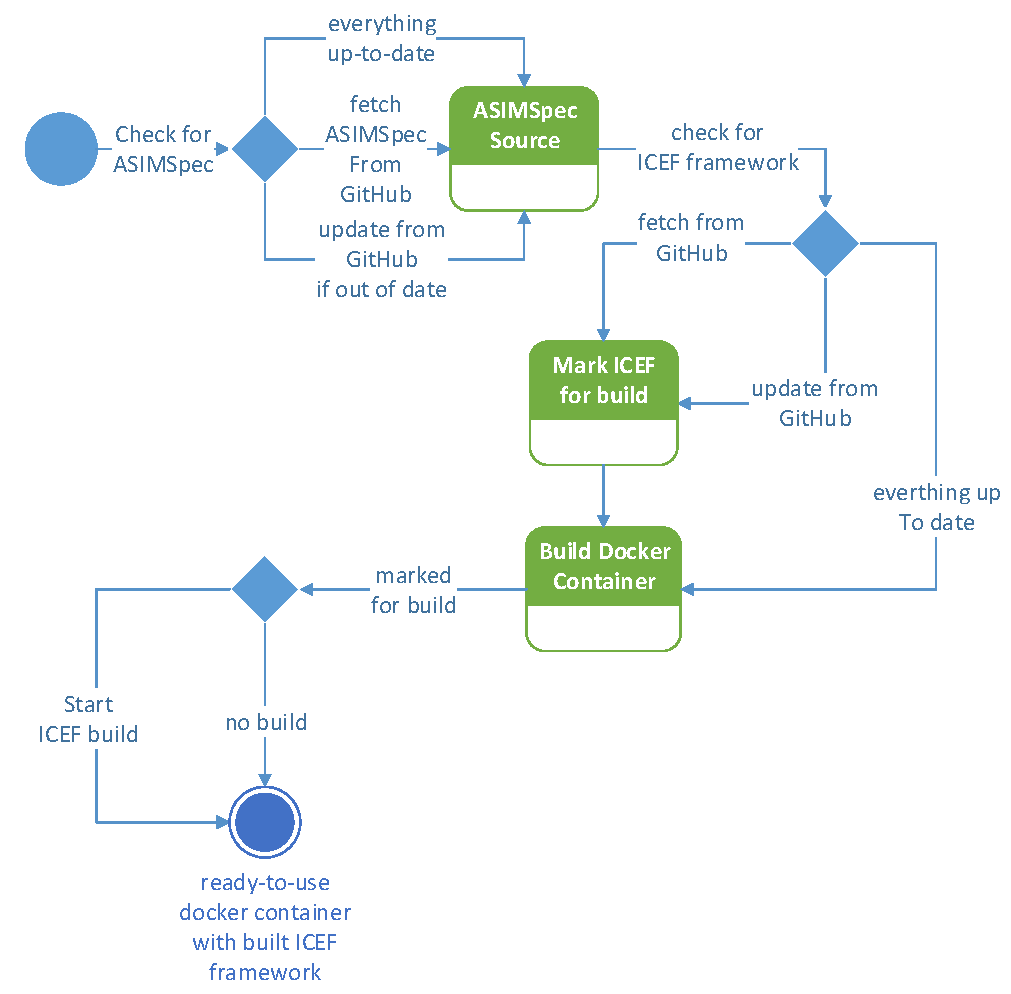
\includegraphics[width=0.8\textwidth, clip, trim=1mm 1mm 1mm 1mm]{Figures/docker_configure}
  \caption{\bf\small Docker Configuration Process}
  \label{fig:docker-env-config-process}
\end{figure}

Summarizing this process, the script tries to fetch the ASIMSpecs as well as ICEF from GitHub, builds the docker container and finally builds the ICEF framework if necessary. The ICEF framework build is done by the bash script in directory \textit{script/buildICEFDocker.sh} and is executed inside the container.

\textbf{Building the docker container} is a core part of this process, in which the most important tools and packages are installed. These software packages are listed in Section \ref{sec:env-exec-stack-software-stack} in detail. Docker uses a file called \textit{Dockerfile}, listed in Figure \ref{fig:docker-env-file-struct}, to know how the container is provisioned. The file contains several commands which are executed in a playbook-like manner to produce a deterministic system environment.

\subsection{Execute ASIM Specifications}

After the environment has been configured the INTERLACE specifications are ready to be executed. This can be done by calling the \textit{execute} script, which starts the prepared docker container and initializes a process illustrated in Figure \ref{fig:docker-env-config-process}.

This process tries to make development as well as instant executing easier by starting a manager, one brapper, and submitting the ICEF definitions using a single script.

\begin{figure}[htbp]
  \centering
  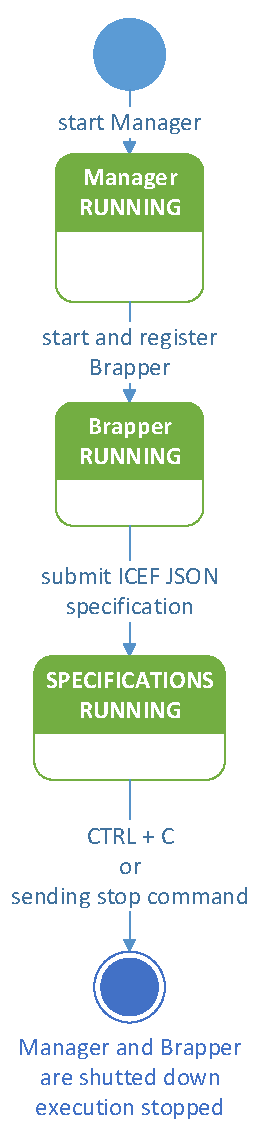
\includegraphics[height=0.9\textwidth, clip, trim=1mm 1mm 1mm 1mm]{Figures/docker_execute}
  \caption{\bf\small Docker Execution Process}
  \label{fig:docker-env-exec-process}
\end{figure}

Note on service locations: In directory \textit{scripts} of Figure \ref{fig:docker-env-file-struct} a file called \textit{asimrc} can be found which acts as a central setup file for configuration and execution and contains the main service locations in the containerized Ubuntu system.

\subsection{Container and Virtual Machine-Based Environments}
Figure \ref{fig:docker-env-container-vs-vm} shows two virtualization techniques. They have similar approaches to how to isolate and allocate resources. However, they function very differently because a container reaches virtualizsation over splitting an operating system resources and a virtual machine virtualizes hardware on which a whole operating system runs.

\begin{figure}[htbp]
  \centering
  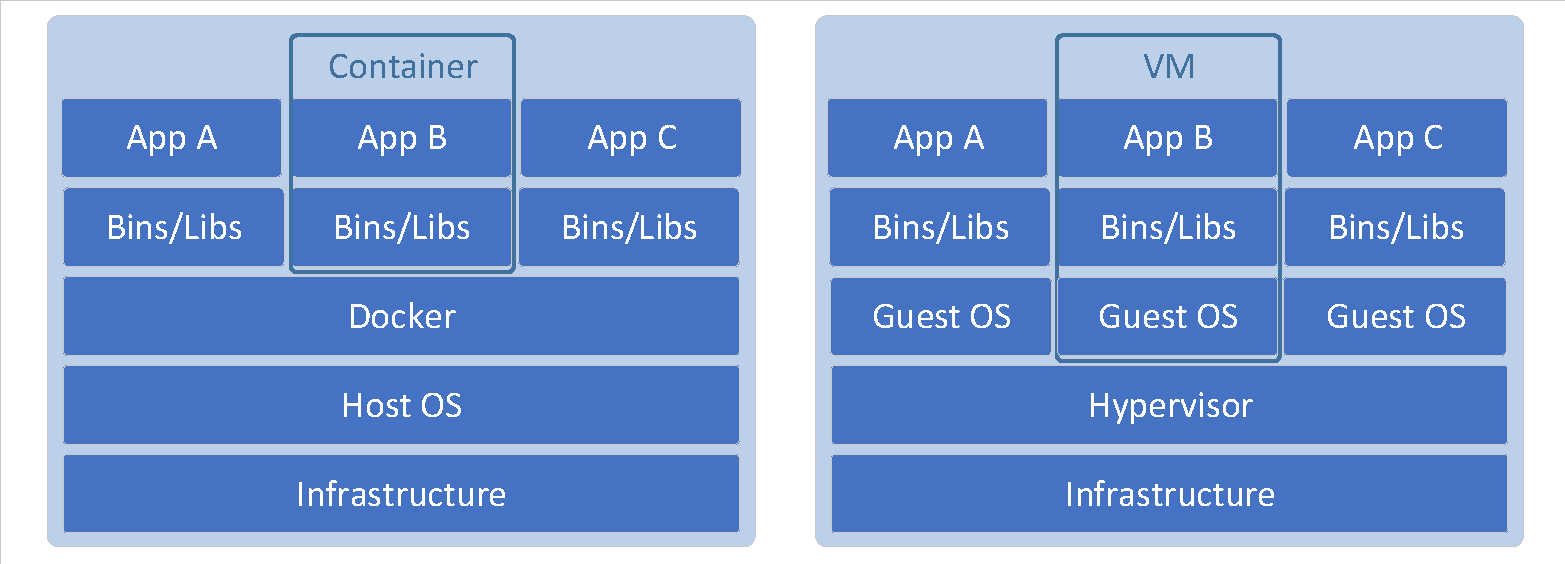
\includegraphics[width=1.0\textwidth, clip, trim=1mm 1mm 1mm 1mm]{Figures/container_vs_vm}
  \caption{\bf\small Container versus Virtual Machine}
  \label{fig:docker-env-container-vs-vm}
\end{figure}

As a consequence, containers can be much smaller, more portable, and in most of the cases also much faster because they are using the system resources more directly and not as wastefully as a virtual machine does.

To be more specific, \textbf{containers} package their libraries and binaries together with an application. Therefore, each container can run in parallel with other containers on the same machine, sharing the OS kernel and each running in an isolated process in user space as if it were a separate OS. Therefore containers have the ability to start instantly, because the operating system they are using is already up and running. Also, they are much smaller as they don't need to carry all the OS-specific software parts.

In contrast, \textbf{virtualized machines} run on an abstraction of the physical hardware which is present in the system. That means that a hypervisor doubles, triples, ... the hardware virtually and allows to install full versions of an operating system compatible with the current system. As each virtualization is a full copy of an OS, images are much larger and boot times most of the time are much slower. Nevertheless, a full operating system might have benefits in some cases over a containerized system.

Coming back to the INTERLACE environments those two approaches reflect the two approaches used for creating the environments. Vagrant is a controlling command line client for hypervisors (virtual machines) and docker is a command line client for a container based virtualization system with the same name.

INTERLACE development efforts are drawn towards the docker environment because execution and starting of the ASIMSpecs is faster and the project is easier to maintain.
